
\documentclass[aspectratio=1610]{beamer}

\usepackage[utf8]{inputenc}
\usepackage[T1]{fontenc}
\usepackage{amsmath,amssymb,amsfonts}
\usepackage{hyperref} % before url package otherwise there is a pb
\usepackage{url}
\usepackage{verbatim}

\usepackage{fontawesome}

\setbeamertemplate{navigation symbols}{%
    \usebeamerfont{footline}%
    \usebeamercolor[fg]{footline}%
    \hspace{1em}%
    \insertframenumber/\inserttotalframenumber
}
\setbeamercolor{footline}{fg=white}

% Dark theme
\setbeamercolor{background canvas}{bg=black}
\setbeamercolor{normal text}{fg=white}
\setbeamercolor{frametitle}{fg=white}
\setbeamercolor{title}{fg=white}
\setbeamercolor{author}{fg=white}
\setbeamercolor{date}{fg=white}
\setbeamercolor{institute}{fg=white}
\setbeamercolor{item}{fg=white}
\setbeamercolor{itemize item}{fg=white}
\setbeamercolor{itemize subitem}{fg=white}
\setbeamercolor{enumerate item}{fg=white}
\setbeamercolor{enumerate subitem}{fg=white}
\setbeamercolor{structure}{fg=white}


\definecolor{btcOrange}{HTML}{F7931A}
\definecolor{ethPurple}{HTML}{627EEA}
\definecolor{solGreen}{HTML}{2A9D8F}
\definecolor{pqRed}{HTML}{E63946}
\definecolor{pqBlue}{HTML}{1D3557}
\definecolor{slipGray}{HTML}{457B9D}
\definecolor{bgLight}{HTML}{F1FAEE}
\definecolor{chainGold}{HTML}{E9C46A}

\usepackage{comment}

\usepackage{algorithmic}
\usepackage[ruled,noline,noend]{algorithm2e}
\algomargin 0pt
\SetAlCapHSkip{0pt}
\DontPrintSemicolon
\SetKw{Continue}{continue}
% fix bug in algorithm2e
\makeatletter
\renewcommand{\@algocf@start}{%
  \@algoskip%
  \begin{lrbox}{\algocf@algobox}%
  \setlength{\algowidth}{\hsize}%
  \vbox\bgroup% save all the algo in a box
  \hbox to\algowidth\bgroup\hbox to \algomargin{\hfill}\vtop\bgroup%
  \ifthenelse{\boolean{algocf@slide}}{\parskip 0.5ex\color{white}}{}%
  % initialization
  \addtolength{\hsize}{-\algomargin}%
  % we don't want our algorithm lines numbered, so let's ditch that right
  % space.
  % \addtolength{\hsize}{-1.5em}% 1.5em to let space for line numbering
  \let\@mathsemicolon=\;\def\;{\ifmmode\@mathsemicolon\else\@endalgoln\fi}%
  \raggedright%
  \AlFnt{}%
  \ifthenelse{\boolean{algocf@slide}}{\IncMargin{\skipalgocfslide}}{}%
  \@algoinsideskip%
%   \let\@emathdisplay=\]\def\]{\algocf@endline\@emathdisplay\nl}%
}%
\makeatother


\SetCommentSty{normalfont}
\SetKwComment{Comment}{$\triangleright$ }{}


\usepackage{tikz}
\usetikzlibrary{calc, positioning, arrows.meta}
\usetikzlibrary{shapes.geometric} % for ellipse
\usetikzlibrary{arrows}
\usetikzlibrary{positioning}
\tikzset{
  state/.style={
    rectangle,
    rounded corners,
    draw=white, thick,
    minimum height=2em,
    inner sep=2pt,
    text centered,
  },
}
\usetikzlibrary{tikzmark}
\usepackage{pgfplots}

\usepackage{multirow}
\usepackage{multicol}

\newcommand{\NN}{\ensuremath{\mathbb N}}
\newcommand{\ZZ}{\ensuremath{\mathbb Z}}
\newcommand{\QQ}{\ensuremath{\mathbb{Q}}}
\newcommand{\RR}{\ensuremath{\mathbb{R}}}
\newcommand{\CC}{\ensuremath{\mathbb{C}}}
\newcommand{\K}{\ensuremath{\mathbb{K}}}
\newcommand{\PP}{\ensuremath{\mathbb{P}}} % for projective line
\newcommand{\FF}{\ensuremath{\mathbb F}}
\newcommand{\F}{\ensuremath{\mathbb F}}
\newcommand{\GG}{\ensuremath{\mathbb G}}
\newcommand{\G}{\ensuremath{\mathbb G}}
\newcommand{\GT}{\ensuremath{\mathbb G_{\text{T}}}}
\newcommand{\Fp}{\F_p}
\newcommand{\cO}{\ensuremath{\mathcal O}}
\newcommand{\cF}{\ensuremath{\mathcal F}}
\DeclareMathOperator{\Norm}{Norm}
\DeclareMathOperator{\ord}{ord}
\DeclareMathOperator{\disc}{Disc}
\DeclareMathOperator{\coeff}{Coeff}
\DeclareMathOperator{\cont}{cont}
\DeclareMathOperator{\reslt}{Res}
\DeclareMathOperator{\Reslt}{Res}
\DeclareMathOperator{\Res}{Res}
\DeclareMathOperator{\val}{val}
\DeclareMathOperator{\GF}{GF}
\DeclareMathOperator{\aut}{aut}
\DeclareMathOperator{\End}{End}
\DeclareMathOperator{\lc}{lc} % for leading coefficient
\DeclareMathOperator{\Id}{Id} % for Identity
\DeclareMathOperator{\Div}{div}
\newcommand{\BLS}{\mbox{BLS}}

\usepackage{fontawesome}
\usepackage{colortbl}
\arrayrulecolor{white}

\date{
  April 1st, 2026\\
  \texttt{EthCC[9]}\\
  Cannes, France
}
\title{
  Future-Proof Your Treasury:\\
  Post-Quantum Accounts for Kohaku Wallet
}
\author{Simon Masson\\

\includegraphics[height=4em]{zknox-logo.png}}
\begin{document}
\begin{frame}
  \maketitle
\end{frame}

\begin{frame}{ZKNOX team}
  \begin{minipage}{.65\linewidth}
   \begin{tabular}{rl}
      \multirow{4}{*}{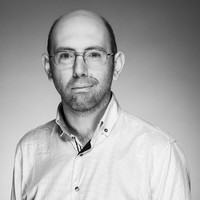
\includegraphics[width=2cm]{NB.jpeg}} & \textbf{Nicolas Bacca}\\
                               & \small{$20^+$ years experience ($10^+$y web3)}\\
                               & Security and hardware specialist\\
                               & \small{Prev.~Ledger cofounder/CTO}\\
                               & \\
      \multirow{4}{*}{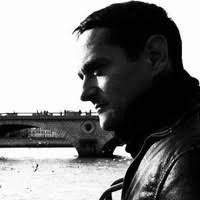
\includegraphics[width=2cm]{RD.jpeg}} & \textbf{Renaud Dubois}\\
                               & \small{$20^+$ years experience ($3^+$y web3)}\\
                               & Cryptographer\\
                               & \small{Prev.~Ledger, Thales}\\
                               & \\
      \multirow{4}{*}{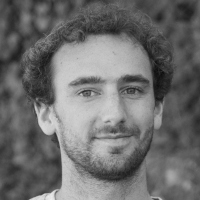
\includegraphics[width=2cm]{SM.jpg}} & \textbf{Simon Masson}\\
                               & \small{$8^+$ years experience ($4^+$y web3)}\\
                               & Cryptographer\\
                               & \small{Prev.~Heliax, Thales}\\
  \end{tabular}
\end{minipage}\pause
\begin{minipage}{.33\linewidth}
   Expertise and innovation to every challenge on the whole security chain:
   \begin{itemize}
   \item user end\\ (secure enclaves, hardware wallets),
   \item back end\\ (TEE, HSMs),
   \item on-chain\\ (smart contracts).
   \end{itemize}

  \pause
 
  \vspace{1em}

  \href{https://zknox.com/}{\texttt{zknox.com}}

\end{minipage}
\end{frame}

\begin{frame}{Kohaku}
  \begin{center}
  
\includegraphics[width=8cm]{kohaku.png}
  \end{center}

  Wallet focusing on privacy and security:
  \begin{itemize}
    \item Overall presentation by N.~Consigny, Monroe Stage (now :-/)
    \item Trustless manifesto by S.~Kux, Taylor Stage (after me ;-))
    \item Privacy integration in hardware wallets by R.~Dubois, Taylor Stage (yesterday)
    \item \textcolor{gray}{Account abstraction targeted soon, enabling integration of this work!}
  \end{itemize}
\end{frame}

\begin{frame}{Why post-quantum?}
  Security of Ethereum relies on \textbf{digital signatures}:
  \begin{itemize}[<+->]
    \item ECDSA: Elliptic Curve Digital Signature Algorithm.
    \item Public key and signature are short (32B to 64B).
    \item Fast to verify, secure, and trusted.
    \item \textcolor{red}{A quantum computer breaks the security!}
    \item Other signatures resist against quantum algorithms.
    \item 2016: NIST starts a standardization process.
    \item 2026: Three candidates for post-quantum secure signature.\\
    Many institutions already integrate PQ security.
  \end{itemize}
\end{frame}

\begin{frame}{Post-quantum signature candidates}
  \begin{center}
    \begin{tabular}{|l|c|c|c|}
      \hline
      Standard &  \textbf{FN-DSA} & \textbf{ML-DSA} & \textbf{SLH-DSA}\\
      Name & Falcon & Dilithium & Sphincs\\
      FIPS &  203 & 204 & 205\\
      Family & Lattice & Lattice & Hash\\
      \hline
      Signature & \uncover<2->{\textcolor{green}{666B} & \textcolor{orange}{2420B} & \textcolor{red}{7856B}}\\
      \hline
      Public key & \uncover<3->{897B & \textcolor{orange}{1312B} & 32B}\\
      \hline
      Gas cost verification & \uncover<4->{\multirow{2}{*}{3.9M} & \multirow{2}{*}{8.1M} & \multirow{2}{*}{--}}\\
      without precompile & \uncover<4->{& &}\\
      \hline
      Hardware  & \uncover<5->{\textcolor{orange}{requires a lot} & \textcolor{green}{yes, see later} & \multirow{2}{*}{--}}\\
      implementation & \uncover<5->{\textcolor{orange}{of RAM}  & \textcolor{green}{in this talk} &}\\
      \hline
      Aggregation & \uncover<6->{eprint 2024/311 & no & no}\\
      \hline
      TSS & \uncover<6->{okay for small $n$ & yes & no}\\
      \hline
      PK recovery & \uncover<6->{yes & no & no}\\
      \hline
    \end{tabular}
  \end{center}
\end{frame}

\begin{frame}{EIP 8051: MLDSA}
  Two precompiles:
  \begin{itemize}
    \item ML-DSA-NIST: using the hash function SHAKE256 (compliant to NIST)
    \item ML-DSA-ETH: using the hash function KECCAK256 (efficient in Ethereum)
  \end{itemize}
  \pause 
  Public key is expanded during verification into ($\mathbb F_q^{4\times 4}, bytes, \mathbb F_q^4$):
  % \begin{center}
  %   \begin{tikzpicture}[
  %     pk/.style={draw=white, text=white, rounded corners, minimum width=1cm, minimum height=.5cm, align=center},
  %     pkexp/.style={draw=white, fill=purple!40, text=white, rounded corners, minimum width=2cm, minimum height=.5cm, align=center},
  %     % verifbox/.style={draw, fill=purple!30, rounded corners, minimum width=2cm, minimum height=.5cm, align=center},
  %     % 4337box/.style={draw, fill=green!30, rounded corners, minimum width=2cm, minimum height=.5cm, align=center},
  %     % boolbox/.style={draw, minimum width=1cm, minimum height=.25cm, align=center},
  %     % arrow/.style={thick, ->, >=Stealth}
  %   ]

  %   % Notes
  %   \onslide<1->{\node[pk] (pk) {Public key\\1312B};}
  %   \onslide<2->{\node[pkexp, right=4cm of pk] (pkexp) {Expanded public key ($\mathbb F_q^{4\times 4}, bytes, \mathbb F_q^4$)\\\textbf{20512B}};}
  %   \onslide<2->{\draw[->, white](pk) -- (pkexp) node[midway, above]{using hash};}
  %   \end{tikzpicture}
  % \end{center}

  \begin{center}
    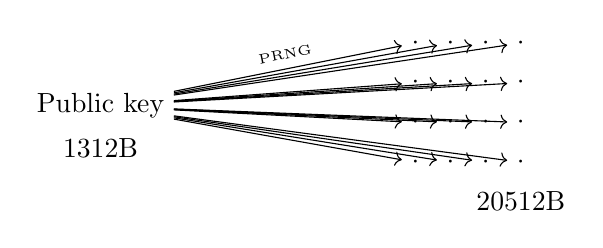
\begin{tikzpicture}
    % Notes
    \node (pk) at (0,0) {Public key};
    \node [below=.01cm of pk] (pksize) {1312B};
    \onslide<2->{
    \node (A00) at (4,.8) {$\cdot$};
    }
    \onslide<3->{
    \node [right=.1cm of A00] (A01) {$\cdot$};
    }
    \onslide<4->{
    \node [right=.1cm of A01] (A02) {$\cdot$};
    }
    \onslide<5->{
    \node [right=.1cm of A02] (A03) {$\cdot$};
    \node [below=.1cm of A00] (A10) {$\cdot$};
    \node [right=.1cm of A10] (A11) {$\cdot$};
    \node [right=.1cm of A11] (A12) {$\cdot$};
    \node [right=.1cm of A12] (A13) {$\cdot$};
    \node [below=.1cm of A10] (A20) {$\cdot$};
    \node [right=.1cm of A20] (A21) {$\cdot$};
    \node [right=.1cm of A21] (A22) {$\cdot$};
    \node [right=.1cm of A22] (A23) {$\cdot$};
    \node [below=.1cm of A20] (A30) {$\cdot$};
    \node [right=.1cm of A30] (A31) {$\cdot$};
    \node [right=.1cm of A31] (A32) {$\cdot$};
    \node [right=.1cm of A32] (A33) {$\cdot$};
    \node [below=.05cm of A33] (pkexpandedsize) {20512B};
    }
    \onslide<2->{
    \draw[->] (pk) -- (A00) node[above, midway, sloped]{{\tiny PRNG}} ;
    }
    \onslide<3->{
    \draw[->] (pk) -- (A01);
    }
    \onslide<4->{
    \draw[->] (pk) -- (A02);
    }
    \onslide<5->{
    \draw[->] (pk) -- (A03);
    \draw[->] (pk) -- (A10);
    \draw[->] (pk) -- (A11);
    \draw[->] (pk) -- (A12);
    \draw[->] (pk) -- (A13);
    \draw[->] (pk) -- (A20);
    \draw[->] (pk) -- (A21);
    \draw[->] (pk) -- (A22);
    \draw[->] (pk) -- (A23);
    \draw[->] (pk) -- (A30);
    \draw[->] (pk) -- (A31);
    \draw[->] (pk) -- (A32);
    \draw[->] (pk) -- (A33);
    }
    \end{tikzpicture}
  \end{center}

  \onslide<6->{Instead of hundreds of hashes, the public key is stored in expanded form in a contract.}
  
  \onslide<7->{Verifier cost: \textbf 9 SHA256 (or \textbf 5 Keccak256) and \textbf{9} NTTs.}
\end{frame}

\begin{frame}{EIP 8052: FNDSA}
  Two precompiles (separation between hash and sign):
  \begin{itemize}
    \item HashToPoint: hashing a message to a polynomial, can be instantiated with different hash functions,
    \item Falcon core verification: verify the shortness of the signature (include NTTs).
  \end{itemize}
  \pause
  Allows different versions of hash functions:
  \begin{itemize}
    \item SHAKE-based: NIST-compliant,
    \item KeccakPRNG-based: gas-efficient.
  \end{itemize}
\end{frame}

\begin{frame}{Account Abstraction}
  \begin{center}
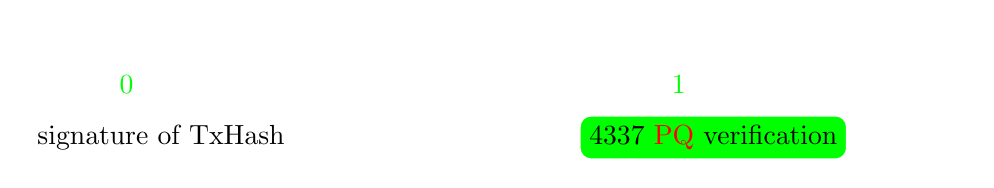
\begin{tikzpicture}[
  note/.style={draw=white, text=white, rounded corners, minimum width=3cm, minimum height=1cm, align=center},
  sigbox/.style={draw=white, fill=white, text=black, rounded corners, minimum width=2cm, minimum height=.5cm, align=center},
  verifbox/.style={draw=white, fill=white, text=black, rounded corners, minimum width=2cm, minimum height=.5cm, align=center},
  4337box/.style={draw=white, fill=green, text=black, rounded corners, minimum width=2cm, minimum height=.5cm, align=center},
  boolbox/.style={draw=white, text=white, minimum width=1cm, minimum height=.25cm, align=center},
  arrow/.style={thick, ->, >=Stealth, white}
]

% Notes
\onslide<1-4>{\node[note] (alice) {Alice \\ 1 ETH};}
\onslide<1-4>{\node[note, right=4cm of alice] (bob) {Bob \\ 0 ETH};}
\onslide<5->{\node[note] (alice) {Alice \\ \textcolor{green}{0} ETH};}
\onslide<5->{\node[note, right=4cm of alice] (bob) {Bob \\ \textcolor{green}{1} ETH};}
\onslide<2->{\draw[->, white](alice) -- (bob) node[midway, above]{Send 1 ETH} node[midway,below]{\texttt{TxHash}: \texttt{0xaf32..ec39}};}
\onslide<3->{\node[sigbox, below=0.1cm of alice] (sig) {signature of TxHash};}
\onslide<4-5>{\node[verifbox, below=0.1cm of bob] (verif) {Verification contract};}
\onslide<5->{\node[boolbox, right=0.5cm of verif] (bool) {True};}
\onslide<5->{\draw[->, white](verif) --  (bool);}
\onslide<6>{\node[4337box, below=0.1cm of bob] (verif) {4337 contract};}
\onslide<7->{\node[4337box, below=0.1cm of bob] (verif) {4337 \textcolor{red}{PQ} verification};}
\end{tikzpicture}
\end{center}

\begin{itemize}
  \onslide<3->{\item Execution layer: ECDSA signature (not resistant to quantum attacks)}
   
  \onslide<6->{\item \textcolor{green}{Account abstraction (4337): enables custom contract for transactions.}}

  \onslide<7->{\item \textcolor{green}{This work: 4337 contract with \textcolor{red}{quantum-secure} signature verification.}}
\end{itemize}
\end{frame}

\begin{frame}{Hybrid verification}
  What is hybrid verification?
  \begin{itemize}
    \item Verify ECDSA signature (Nowadays security and trust),
    \item Verify PQ signature (security against a quantum computer).
  \end{itemize}
  $\Longrightarrow$ Nowadays trust and future quantum security.
  \pause

  \begin{itemize}
    \item Pre-quantum:
    \begin{itemize}
      \item ECDSA-k1 (signature in Ethereum standard transaction),
      \item ECDSA-r1 (signature for passkey).
    \end{itemize}
    \pause
    \item Post-quantum:
    \begin{itemize}
      \item MLDSA (NIST standard),
      \item MLDSA-ETH (gas efficient variant),
      \item FALCON (NIST standard),
      \item FALCON-ETH (gas efficient variant).
    \end{itemize}
  \end{itemize}
\end{frame}

\begin{frame}{Smart Account Contract}
    \begin{algorithmic}
      \STATE \texttt{SigContract1 = SigVerifier(LogicAddress1)}
      \hfill \Comment{\textcolor{gray}{pre-quantum signature verifier}}
      \pause
      \IF {\texttt{not(SigContract1.verify(PubKey1, digest, Sig1))}}
      \RETURN \texttt{\textcolor{red}{False}}
      \ENDIF
      \pause

      \STATE \texttt{SigContract2 = SigVerifier(LogicAddress2)}
      \hfill \Comment{\textcolor{gray}{post-quantum signature verifier}}
      \pause
      \IF {\texttt{not(SigContract2.verify(PubKey2, digest, Sig2))}}
      \RETURN \texttt{\textcolor{red}{False}}
      \ENDIF
      \pause

      \RETURN \texttt{\textcolor{green}{True}}
  \end{algorithmic}
  \pause

  \begin{itemize}[<+->]
    \item Modular: interface verifiers are provided with the account factory
    \item Possible to use two PQ verifiers {\tiny if you don't know which one to choose ;-)},
    \item Practical gas costs (without precompile):
    \begin{itemize}[<0->]
      \item ECDSA + MLDSA: 8.39M gas,
      \item ECDSA + FALCON: 4.06M gas,
      \item ECDSA + MLDSA-ETH: 5.12M gas,
      \item ECDSA + ETH-FALCON: 1.69M gas.
    \end{itemize}
  \end{itemize}
\end{frame}

\begin{frame}{PQ-SLIP: how to handle PQ keys}

\centering
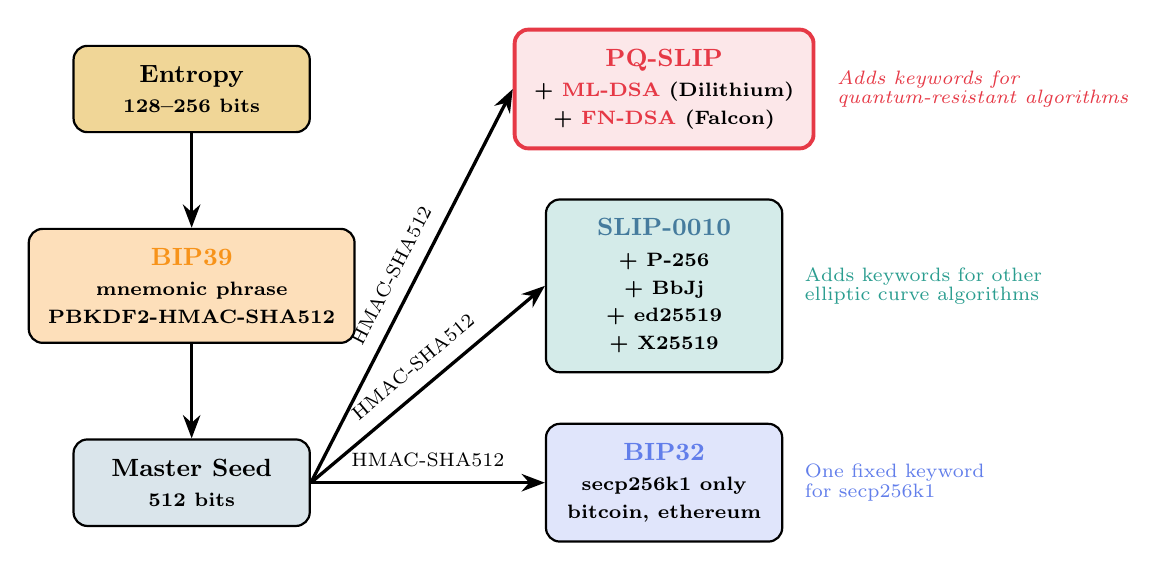
\begin{tikzpicture}[
  box/.style      = {rounded corners=5pt, black, draw, thick, align=center,
                     inner sep=7pt, font=\small\bfseries, minimum width=3.0cm},
  smallbox/.style = {rounded corners=4pt, draw, thick, align=center,
                     inner sep=5pt, font=\scriptsize\bfseries, minimum width=2.6cm},
  arrow/.style    = {-Stealth, line width=1.2pt},
  darrow/.style   = {-Stealth, line width=1pt, dashed},
  lbl/.style      = {font=\scriptsize, midway},
]

% A: Entropy  (top-left)
\node[box, fill=chainGold!70] (entropy) at (0, 0)
  {Entropy \\ \scriptsize 128--256 bits};

% B: BIP39  (bottom-left)
\node[box, fill=btcOrange!30] (bip39) at (0, -2.5)
  {\textcolor{btcOrange}{BIP39} \\
   \scriptsize mnemonic phrase \\[-1pt]
   \scriptsize PBKDF2-HMAC-SHA512};

% C: Master Seed  (bottom-centre)
\node[box, fill=slipGray!20] (seed) at (0,-5)
  {Master Seed \\ \scriptsize 512 bits};

  \onslide<2->{
% C1: BIP32 side-branch below Seed
\node[box, fill=ethPurple!20] (bip32) at (6, -5)
  {\textcolor{ethPurple}{BIP32} \\
   \scriptsize secp256k1 only \\[-1pt]
   \scriptsize bitcoin, ethereum};
  }

  \onslide<3->{
% C2: SLIP-0010  (bottom-right)
\node[box, fill=solGreen!20] (slip) at (6, -2.5)
  {\textcolor{slipGray}{\textbf{SLIP-0010}} \\
   \scriptsize + P-256\\[-1pt]
   \scriptsize + BbJj\\[-1pt]
   \scriptsize + ed25519\\[-1pt]
   \scriptsize + X25519};
  }

  \onslide<4->{
% C3: PQSLIP  (top-right)
\node[box, fill=pqRed!12, draw=pqRed, line width=1.4pt] (pqslip) at (6.0, 0)
  {\textcolor{pqRed}{\textbf{PQ-SLIP}} \\
   \scriptsize + \textcolor{pqRed}{\textbf{ML-DSA}} (Dilithium) \\[-1pt]
   \scriptsize + \textcolor{pqRed}{\textbf{FN-DSA}} (Falcon)};
  }

% A -> B (mid)
\draw[arrow] (entropy.south) -- (bip39.north);

% B -> C (down)
\draw[arrow] (bip39.south) -- (seed.north);

\onslide<2->{
% C -> C1 (right down)
\draw[arrow] (seed.east) -- (bip32.west)
  node[lbl, above=2pt, sloped] {\scriptsize HMAC-SHA512};
}

\onslide<3->{
% C -> C2 (right mid)
\draw[arrow] (seed.east) -- (slip.west)
  node[lbl, above=2pt, sloped] {\scriptsize HMAC-SHA512};
}

\onslide<4->{
% C -> C3 (right up)
\draw[arrow] (seed.east) -- (pqslip.west)
  node[lbl, above=2pt, sloped] {\scriptsize HMAC-SHA512};
}

% Labels
\onslide<2->{
\node[font=\scriptsize, right=0.15cm of bip32, text=ethPurple, align=left]
  {One fixed keyword\\[-1pt]for secp256k1};
}

\onslide<3->{
\node[font=\scriptsize, right=0.15cm of slip, text=solGreen, align=left]
  {Adds keywords for other\\[-1pt]elliptic curve algorithms};
}

\onslide<4->{
\node[font=\scriptsize\itshape, right=0.15cm of pqslip, text=pqRed, align=left]
  {Adds keywords for\\[-1pt]quantum-resistant algorithms};
}

\end{tikzpicture}

\end{frame}


\begin{frame}{Demonstration: what do we show here?}
  \begin{description}[<+->]
    \item [Step 1.] Create Account
    \begin{itemize}[<0->]
      \item \textcolor{gray}{Requires an EOA that is already funded},
      \item Derive pre-quantum and post-quantum seed,~\onslide<3->{\textcolor{red}{HW or SW}}
      \item Pre-quantum key generation: $(\mathbf{sk}_1,\mathbf{pk}_1)$,~\onslide<3->{\textcolor{red}{HW or SW}}\\
      Post-quantum key generation: $(\mathbf{sk}_2,\mathbf{pk}_2)$,~\onslide<3->{\textcolor{red}{HW or SW}}
      \item \emph{The account is created} as a 4337 smart contract storing $\mathbf{pk}_1$ and $\mathbf{pk}_2$.
    \end{itemize}
    \item [Step 2.] Send Transaction
    \begin{itemize}[<0->]
      \item \textcolor{gray}{Does not require an EOA anymore},
      \item \textcolor{gray}{The freshly created account needs to be funded},
      \item Compute the \texttt{UserOpHash} to be signed,~\onslide<4->{\textcolor{green}{HW or SW (clear signing)}}
      \item Sign it with a pre-quantum scheme using $\mathbf{sk}_1$,~\onslide<3->{\textcolor{red}{HW or SW}}\\
      Sign it with a post-quantum scheme using $\mathbf{sk}_2$,~\onslide<3->{\textcolor{red}{HW or SW}}
      \item \emph{A transaction is spent} from the 4337 account if:
      \begin{itemize}
        \item the pre-quantum signature is valid w.r.t~$\mathbf{pk}_1$ stored in the contract,
        \item the post-quantum signature is valid w.r.t~$\mathbf{pk}_2$ stored in the contract,
      \end{itemize}
    \end{itemize}
  \end{description}
  \begin{center}
    \onslide<5->{
      \textbf{\textcolor{blue}{https://pq4337.netlify.app/}}
    }
  \end{center}
\end{frame}

\begin{frame}{Conclusion and perspectives}
  Smart accounts with post-quantum security are already available!
  \begin{itemize}
    \item[\faCheckSquareO] Experimentation with MLDSA and FALCON: decent cost for L2
    \item[\faSquareO] Production: audit of the code is missing
    \pause
    \item[\faCheckSquareO] Hardware: MLDSA available (in hybrid)
    \item[\faSquareO] Hardware: FALCON requires a lot of memory
    \pause
    \item[\faClockO] L1 is waiting for a precompile:
    \begin{itemize}
      \item EIP-8051,
      \item EIP-8052,
      \item EIP-7885 (NTT) + hash precompile,
      \item Vectorized arithmetic precompile.
    \end{itemize}
    \pause
    \item[\faSquareO] Delegation (7702) and deactivation of EOA (7851) is not implemented yet
  \end{itemize}

  \pause
  \textcolor{green}{BONUS}: a NFT offered to the first to create a PQ account and sends some ETH to \texttt{zknox.eth} on Sepolia! ;-)

\end{frame}

% \begin{frame}{Hardware implementation}
%   \begin{itemize}[<+->]
%     \item Start from NIST FIPS 204 reference code
%     \begin{center}
%       
\includegraphics[width=5cm]{nist-github.png}
%     \end{center}
%     \item Adaptations for low ram constraints:
%     \begin{center}
%       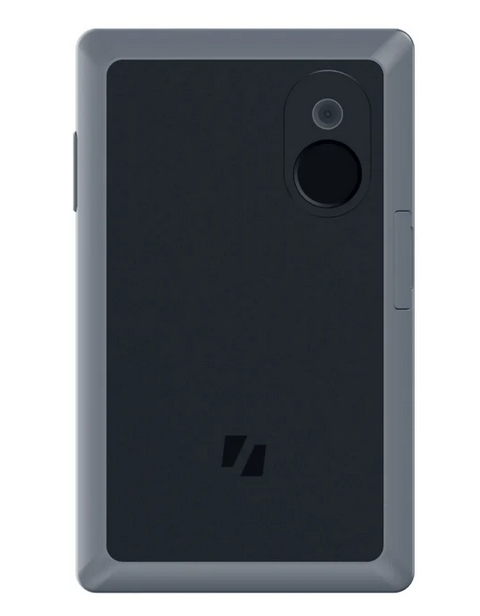
\includegraphics[scale=.25]{keystone.png}
%       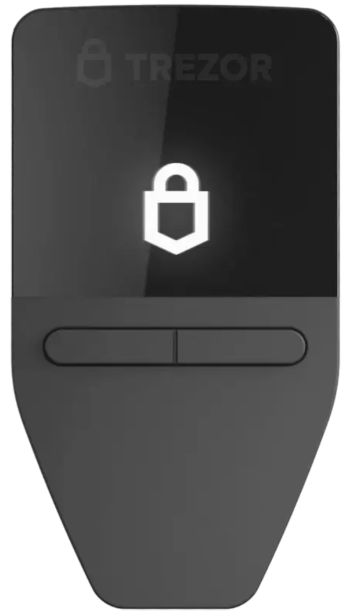
\includegraphics[scale=.25]{trezor.png}
%       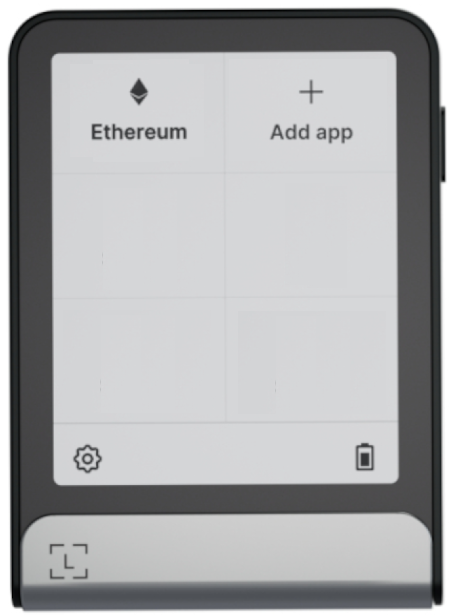
\includegraphics[scale=.25]{flex.png}
%     \end{center}
%     \item Ledger RAM $\leq 50$kB $\Rightarrow$ implem.~as in ia.cr/2022/323 (thanks to \texttt{dop-amin})
%     \item Entire computation in the Secure Element (the secret never leaves the enclave)
%     \item Provide two signers for the two precompiles:
%     \begin{itemize}
%       \item MLDSA (SHAKE256 using NIST code) signing in 700ms,
%       \item MLDSA-ETH (Keccak256 BOLOS calls) signing slower (BOLOS communication).
%     \end{itemize}
%     \item Implementation tricks:
%     \begin{itemize}
%       \item Recomputation of keygen to save RAM access,
%       \item Tweaked BIP32 to derive unique secret per hardware
%       \item Public key (resp.~signature) fetching requires 6 APDUs (resp.~10 APDUs) to get 255B chunks
%     \end{itemize}
%     \item Soon on other HW...
%   \end{itemize}
% \end{frame}


% \begin{frame}{Hybrid 4337}
%   \begin{itemize}[<+->]
%     \item MLDSA Expanded public key stored on-chain (20512B) per user
%     \item Hybrid contract:
%     \begin{enumerate}
%       \item Fetches the MLDSA public key
%       \item Verifies the Post-Quantum signature
%       \item Fetches the ECDSA public key (or Ethereum address)
%       \item Verifies the ECDSA signature using \texttt{ecrecover}
%       \item Accepts only if \textbf{both} signatures are valid.
%     \end{enumerate}
%   \end{itemize}

%     \begin{center}
%       \begin{tikzpicture}[
%         note/.style={draw=white, text=white, rounded corners, minimum width=3cm, minimum height=1cm, align=center},
%         sigbox/.style={draw=white, fill=purple!40, text=white, rounded corners, minimum width=2cm, minimum height=.5cm, align=center},
%         sigbox2/.style={draw=white, fill=purple!40, text=white, rounded corners, minimum width=2cm, minimum height=.5cm, align=center},
%         verifbox/.style={draw=white, fill=purple!50, text=white, rounded corners, minimum width=2cm, minimum height=.5cm, align=center},
%         4337box/.style={draw=white, fill=green!40, text=black, rounded corners, minimum width=2cm, minimum height=.5cm, align=center},
%         boolbox/.style={draw=white, text=white, minimum width=1cm, minimum height=.25cm, align=center},
%         arrow/.style={thick, ->, >=Stealth, white}
%       ]

%       % Notes
%       \onslide<8-9>{
%         \node[note] (alice) {Alice \\ 1 ETH};
%         \node[note, right=4cm of alice] (bob) {Bob \\ 0 ETH};
%       }
%       \onslide<10->{
%         \node[note] (alice) {Alice \\ \textcolor{green}{0} ETH};
%         \node[note, right=4cm of alice] (bob) {Bob \\ \textcolor{green}{1} ETH};
%       }
%       \onslide<8->{
%         \draw[->, white](alice) -- (bob) node[midway, above]{Send 1 ETH} node[midway,below]{\texttt{TxHash}: \texttt{0xaf32..ec39}};
%       }
%       \onslide<9->{
%         \node[sigbox, below=0.1cm of alice] (sig) {EC sig of TxHash};
%         \node[sigbox2, below=0.1cm of sig] (sigpq) {ML sig of TxHash};
%       }
%       \onslide<10->{
%         \node[4337box, below=0.1cm of bob] (verif) {4337 contract};
%         \node[boolbox, right=2cm of verif] (bool) {True};
%         \draw[->, white](verif) --  (bool) node[midway, above]{verif EC?} node [midway, below]{verif ML?};
%       }
%     \end{tikzpicture}
%   \end{center}
%   \onslide<11->{
%     Thanks to Alex and Shahaf from 4337 team for the integration help :-)
%   }
% \end{frame}

% \begin{frame}{Conclusion and perspectives}
%  \begin{itemize}[<+->]
%   \item[$\checkmark$] Hardware implementation of MLDSA and MLDSAETH,
%   \item[$\checkmark$] Hybrid 4337 account with ECDSA and MLDSA,
%   \item [$\Box$] BIP32 compliant secret derivation,
%   \item [$\Box$] Universal Ethereum app enables FN-DSA and ML-DSA on other HW,
%   \item [$\Box$] More comparisons with FN-DSA,
%   \item [$\Box$] Experiments on L2 possible but gas is expensive.
%   \end{itemize}
%   \begin{flushright}
%   \onslide<7>{Thank you for your attention.}
%   \end{flushright}
% \end{frame}


\end{document}
